\documentclass[10pt]{beamer}
\usepackage[utf8]{inputenc}
\usepackage{graphicx}
\usepackage[T1]{fontenc}
\usepackage{enumitem}
\usepackage{siunitx}
\usepackage{pifont}
\usepackage{stanli}
\usepackage{varwidth}
\usepackage{tikz}
\usepackage[outdir=convertedFigs/]{epstopdf}
\usepackage{animate}
\usepackage{pgfplots}
\usepackage[export]{adjustbox}
\usepackage{copyrightbox}
\usepackage{lastpage}
\usepackage{subfig}
\usetikzlibrary{positioning}
\usetikzlibrary{calc}
\pgfplotsset{compat=1.11}
\usetikzlibrary{shadows}
\usepackage{lastpage}
\usepackage{newunicodechar}
\usepackage{tikzsymbols} 




% Custom Commands
\newcommand{\OK}{\color{green}\ding{52}\color{black}}
\newcommand{\KO}{\color{red}\ding{55}\color{black}}
\newcommand\deriv{\mathrm{d}}
\newcommand\expo[1]{\mathop{\mathrm{e}^\mathrm{#1}}}
\newcommand\Warning{%
	\makebox[1.4em][c]{%
		\makebox[0pt][c]{\raisebox{.1em}{\small!}}%
		\makebox[0pt][c]{\color{red}\Large$\bigtriangleup$}}}%



\begin{document}
	
	%% Entries for Front Page %%
	\title{Génération de signaux \\ aléatoires multi-nodaux inter-corrélés}
	\institute[Séminaire SSD 17/04/20]{Séminaire SSD}
	\author{\begin{tabular}{c} \underline{Julien Heremans} \\ {Vincent Denoël}\end{tabular}}
	\date{\scriptsize 17 avril 2020}
	\def\confLogo{logos/uliege.png}
	
	% Input template
		%% List of Packages to be included %%
%	\usepackage{tikz}
%	\usepackage{varwidth}
%	\usepackage{enumitem}
%	\usepackage{pifont}
%	\usetikzlibrary{positioning}
%	\usetikzlibrary{calc}
%% List of Packages to be included %%



% Change default setup:
\setbeamercovered{transparent}
\setbeamertemplate{navigation symbols}{}


% Change default color:
\definecolor{MyColor}{rgb}{0.9297,0.5351,0.265312} 


%% Modifier le format de la police	
\setbeamerfont{title}{size=\Large}
\setbeamerfont{frametitle}{size=\Large}
\setbeamerfont{framesubtitle}{size=\scriptsize}
\setbeamerfont{institute}{size=\scriptsize}
\setbeamerfont{date}{size=\scriptsize}
\setbeamerfont{author}{size=\normalsize}


% Modifier couleur par défaut:
\setbeamercolor{title}{fg=MyColor}
\setbeamercolor{frametitle}{fg=MyColor}


% Custom environment
\newenvironment{changemargin}[2]{%  
	\begin{list}{}{%
			\setlength{\topsep}{0pt}%
			\setlength{\leftmargin}{#1}%
			\setlength{\rightmargin}{#2}%
			\setlength{\listparindent}{\parindent}%
			\setlength{\itemindent}{\parindent}%
			\setlength{\parsep}{\parskip}%
			\setlength{\topmargin}{-2cm}
		}%
		\item[]}{\end{list}
}


% Custom bullets for itemize labels
\newcommand{\MyShadow}[1]{\tikz{\shade[ball color=MyColor, preaction={fill=black,
			opacity=.35,transform canvas={xshift=1.3mm,yshift=-1.15mm, yscale=0.28}}] (0,0) circle (#1ex);} }
\newcommand*{\itemOneA}{\MyShadow{0.7} }
\newcommand*{\itemOneB}{\MyShadow{0.5} }
\setlist[itemize]{label=\itemOneA}


% Change defaut presentation front page
\def\sizLRat{0.3}
\def\sizTRat{0.7}
\def\sizL2Rat{0.5}
\setbeamertemplate{title page}
{ 	\vspace{-0.08cm}
	\def\pp{0.79\paperwidth} 
	\begin{changemargin}{-1cm}{0cm}
		\begin{tikzpicture}
		\draw [anchor=north west](current page.north west) node  [inner sep=0pt] (pic) {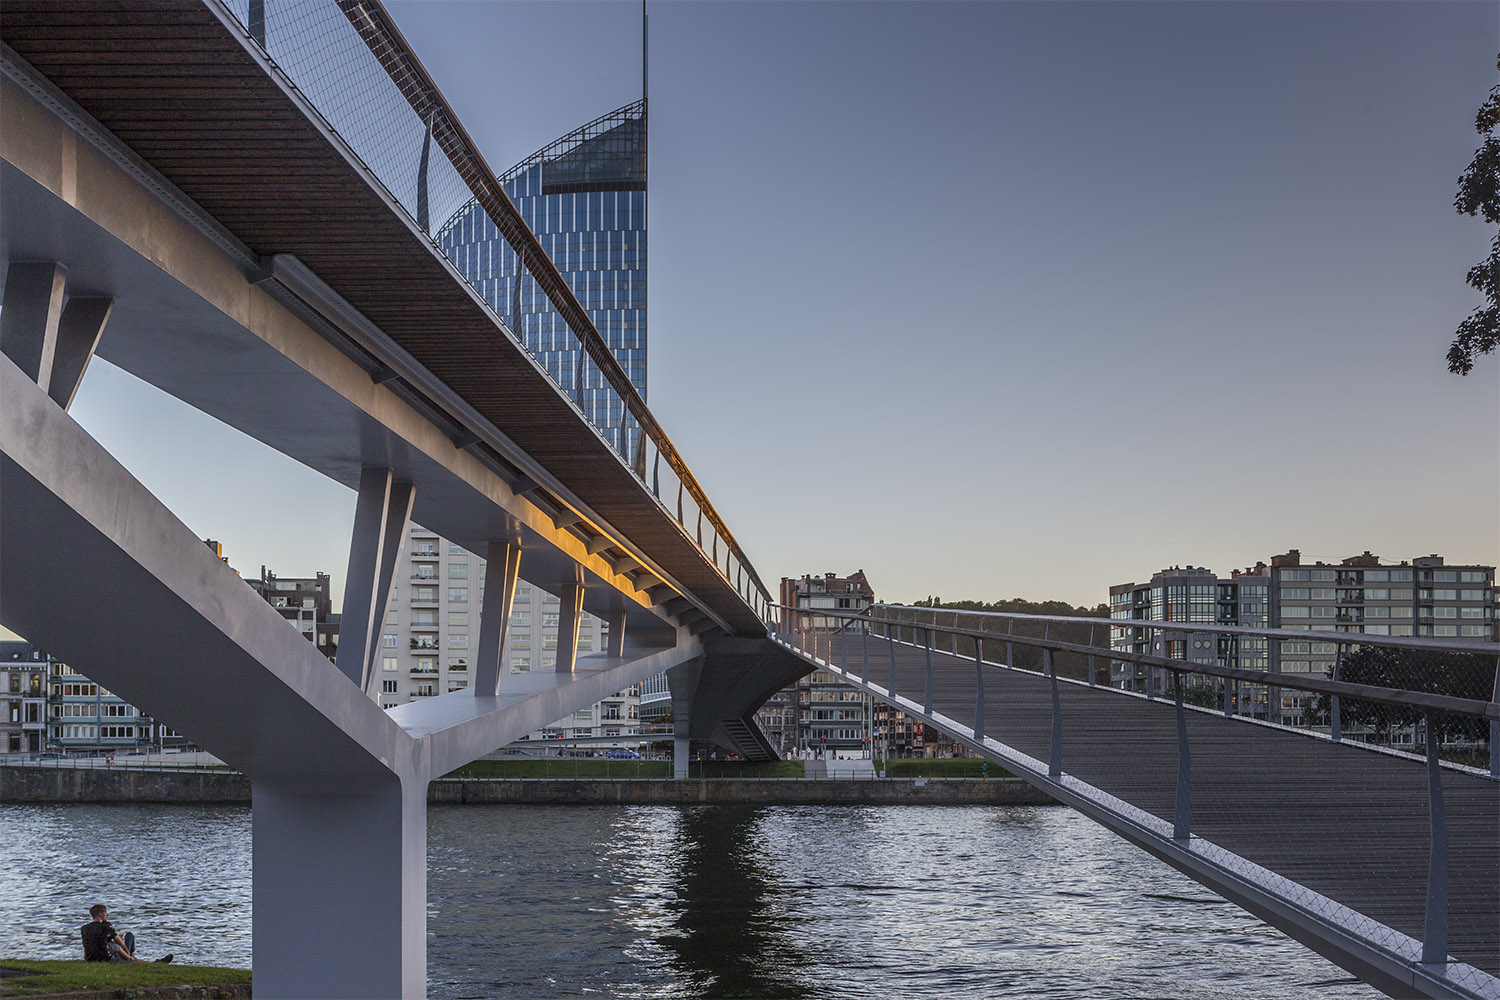
\includegraphics[width=\pp]{logos/image} } ;
		\coordinate (A) at (current page.south west) ;
		\coordinate (TL) at (current page.north west);
		\coordinate (D) at (current page.north east) ;
		\coordinate (E) at (current page.south east) ;
		\path (TL) --  coordinate [pos=\sizTRat] (B) (A) ;
		\path (TL) --  coordinate [pos=\sizTRat] (C) (D) ; 
		\fill [white] (A)--(B)--(C)--(D)--(E) ;
		\node[anchor=north east,xshift=-4pt,yshift=-4pt,align=right] at (current page.north east) {{
\includegraphics[width=0.25\paperwidth]{logos/facsa.pdf}}};
		\node[anchor=north east,xshift=-4pt,yshift=-35pt,align=right] at (D) {{
\includegraphics[width=0.37\paperwidth]{logos/logostocha} }};
		\node [anchor=north, text width=9cm,align=center,color=MyColor,minimum width=8cm] (titre) at (0.65\paperwidth,0.65\paperheight) { \hyphenchar\font=-1
			\usebeamerfont{title}\inserttitle\par} ;
		\node [anchor=north,below=0cm of titre,yshift=-15pt] (autr){\usebeamerfont{author}\insertauthor\par};
		\path (A) -- (TL) coordinate [pos=\sizL2Rat] (B') ;
		\path (A) -- (E) coordinate [pos=\sizTRat] (F) ;
		\fill [gray!10,fill opacity=0.8] (A) -- (B') -- (F) -- cycle ;
		%		\node [inner sep=4pt,anchor=west] (conf)  at (0,0.1\paperheight) { \usebeamerfont{institute}\insertinstitute\par } ;
		\node [inner sep=5pt,anchor=south west,color=MyColor] (date) at (current page.south west) {\usebeamerfont{date}\insertdate\par }; 
		\node [anchor=west, inner sep=5pt,yshift=10pt,color=MyColor](date) at (0,0.05\paperheight) {\insertinstitute};
		\node [anchor=west,inner sep=20pt] at (0,0.22\paperheight) { \includegraphics[width=0.3\paperwidth]{\confLogo} };
		\node [anchor=south east,inner sep = 5pt] at (current page.south east) {{ 
\includegraphics[width=0.2\paperwidth]{logos/uee}}}  ;
		\end{tikzpicture}
	\end{changemargin}
	
	
}


% Change default frame title
\setbeamertemplate{frametitle}
{
	\vspace{0.3cm}\hspace{-0.8cm}
	\begin{tikzpicture}
	\node [color=MyColor,anchor=west] (A) at (0,0) {\begin{varwidth}{0.67\paperwidth} \bfseries \insertframetitle{} 	\end{varwidth}} ;
	\draw (A.south west) coordinate (B) [line width=0.6pt,color=MyColor]-- (A.south east);
	\draw [fill=MyColor, draw=MyColor] (B) circle(1.4pt) {};
	\coordinate (C) at (B.south west) ;
	\draw [anchor=west, color=MyColor] (B) node [yshift=-10pt] {\usebeamerfont{subtitle}\insertframesubtitle{}} ;
	\end{tikzpicture}
	\vspace{-0.2cm}
	\begin{tikzpicture}[remember picture,overlay]
	\node[anchor=north east,xshift=-4pt,yshift=-4pt] at (current page.north east) {
\includegraphics[width=0.25\paperwidth]{logos/facsa.pdf}};
	%	\node [anchor=south east,inner sep = 5pt] at (current page.south east) {{ 
\includegraphics[width=0.2\paperwidth]{logos/uee}}}  ;
	\coordinate (A) at (current page.south west) ;
	\coordinate (TL) at (current page.north west);
	\coordinate (D) at (current page.north east) ;
	\coordinate (E) at (current page.south east) ;
	\path (A) -- (TL) coordinate [pos=\sizL2Rat] (B') ;
	\path (A) -- (E) coordinate [pos=\sizTRat] (F) ;
	\fill [gray!5,fill opacity=0.8] (A) -- (B') -- (F) -- cycle ;
	\node [anchor=south east,inner sep = 5pt,yshift=0pt] at (current page.south east) {\color{black}\scriptsize \insertframenumber{} /\inserttotalframenumber}  ;
	\node [anchor=south west] at (current page.south west) {\color{MyColor}\scriptsize \insertshortinstitute} ;
	\end{tikzpicture}
}



% Add title frame at each new section:
\AtBeginSection[]{
	\begin{frame}
	\vfill
	\centering
	%	\begin{beamercolorbox}[sep=8pt,center,shadow=true,rounded=true]{title}
	%		\usebeamerfont{title}\insertsectionhead\par%
	\begin{tikzpicture}[remember picture,overlay]
	\node[anchor=north east,xshift=-4pt,yshift=-4pt] at (current page.north east) {
\includegraphics[width=0.25\paperwidth]{logos/facsa.pdf}};
	\node [anchor=south east,inner sep = 5pt,yshift=0pt] at (current page.south east) {\color{black}\scriptsize \insertframenumber{} /\inserttotalframenumber}  ;
	\node [anchor=south west] at (current page.south west) {\color{MyColor}\scriptsize \insertshortinstitute} ;
	\node [color=MyColor,anchor=center,align=center] (A) at (0,0) { \usebeamerfont{title} \Large \bfseries  \thesection~-~\insertsection~};
	\coordinate  [yshift=-5pt,xshift=-10pt] (B) at (A.south west) ;
	\coordinate  [yshift=-5pt,xshift=10pt] (C) at (A.south east) ; 
	\draw  [line width=0.9pt,color=MyColor] (B) -- (C);
	\draw [fill=MyColor, draw=MyColor] (B) circle(1.8pt) {};
	\draw [fill=MyColor, draw=MyColor] (C) circle(1.8pt) {};
	\end{tikzpicture}
	%	\end{beamercolorbox}
	\vfill
\end{frame}
}



% Change defaut table of content
\definecolor{itemizecolor}{rgb}{0.18,0.22,0.60}
\defbeamertemplate{section in toc}{square unnumbered}{%
\leavevmode\leftskip=1.75ex%
\llap{{\thesection}}%
\kern1.5ex\inserttocsection\par}
\defbeamertemplate{subsection in toc}{square unnumbered}{%
\leavevmode\leftskip=4.6ex%
\llap{{\color{MyColor}\tiny$\blacksquare$\normalsize}}%
\kern1.5ex\inserttocsubsection\par}
\setbeamertemplate{section in toc}[square]
\setbeamertemplate{subsection in toc}[square unnumbered]




	
	
	% Page de garde
	\begin{frame}[plain]
	\maketitle
	\end{frame}




	% Table des matières
	\begin{frame}
	\frametitle{Table des matières}
	\tableofcontents
	\end{frame}

	% Corps de texte
	\section{First section} % new section name will be displayed in a dedicated headsectionframe + in table on contents
	\subsection{First Subsection} % subsections will be included in table of contents
	
	\begin{frame}
	\frametitle{First Title}
	\framesubtitle{Sub-title}
	
	\begin{itemize}[label=\itemOneA]
	\item Thing 1
	\item Thing 2
	\begin{itemize}[label=\itemOneB]
		\item Subitem
		\item Subitem
	\end{itemize}
	\end{itemize}
	
	\end{frame}


\end{document}